\documentclass{article}
\usepackage[english,polish]{babel}
\selectlanguage{polish}

\title{\huge  \Huge \textbf{MOZA Projekt} \\ \textbf{Wzmacniacz Kaskodowy 4 (wariant B)}}
\date{\today}
\author{ \LARGE Jakub Półtorak}

\usepackage{amsmath}
\usepackage{amsfonts}
\usepackage{graphicx}
\usepackage[T1]{fontenc}
\usepackage{pdflscape}
\usepackage{rotating}

\begin{document}
\maketitle
\pagenumbering{gobble}
\newpage
\pagenumbering{arabic}
\tableofcontents

\pagebreak

\begin{center}
	\title{ \huge \textbf{Etap 1}}
\end{center}


\section{Opis problemu}
Zadanie polega na doborze wartości elementów wzmacniacza tak, aby uzyskać makymalnie duży iloczyn
GBW. Na układ nałożono dodatkowe ograniczenia w postaci minimalnego wzmocnienia dla małych częstotliwości $k_{u0} > 10 dB$ oraz minimalnej częstotliwości
granicznej $f_g > 200 MHz$ (rozumianej jako częstoliwość spadku o 3 dB względem $k_{u0}$).
\section{Sformułowanie matematyczne zadań optymalizacji}
Poszukiwane jest minimum funkcji celu:
\[ \min\limits_{x_1,\dots x_T} f(x) \]
p.o.
\[ g_{i}(\textbf{x}) \leq 0 \ \ \ \  i=1..n_g\]
gdzie:
\[ f(\textbf{x}) = -(k_{u0}\cdot f_g)\]
\(\textbf{x}\) - wektor zmiennych optymalizowanych: \\
\begin{center}
	$\textbf{x}$ =
	$\begin{bmatrix}
			REE1 & REE2 & RE & RC2 & RC3 & CEE & CG
		\end{bmatrix}$,
\end{center}
\(k_{u0}\) - wzmocnienie dla małych częstoliwości, rozumiane jako wzmocnienia dla częstoltiwości 1 kHz.\\
\(f_{g}\) - częstoliwość graniczna, rozumiana jako częstotliwość, dla której wzmocnienie
spada o 3 dB względem $k_{u_{0}}(\textbf{x}) $.

Parametry $k_{u0}(\textbf{x})$ oraz $f_g(\textbf{x})$ obliczane są w Matlabie na pdostawie surowych danych ($U^{AC}_{out}(x,f)$) zwaracnych
przez symulator LTSpice.

Dodatkowo, w zadaniu pojawiają się ogarniczenia nieliniowe związane z wymaganiami projektowymi:\\
\begin{itemize}
	\item \(g_1(\textbf{x}): -(\frac{k_{u0}(\textbf{x})}{k_{u_{min}}}-1) <  0\) \\ Warunek minimalnego wzmocnienia, $k_{umin}=20dB$
	\item \(g_2(\textbf{x}): -(\frac{{f_g}(\textbf{x})}{f_{g_{min}}}-1)<0\) \\ Warunek minimalnej częstotliwości granicznej, $f_{gmin}=200 MHz$
	\item \(g_3(\textbf{x}): b(\textbf{x})-b_{max}<0\) \\ Ograniczenie podbicia charakterystyki, $b_{max}=1dB$. Podbicie $b$ rozumiane jest jako różnica między maksymalnym poziomem wzmocnienia a $k_{u0}$.Podbicie jest obliczane w Matlabie.

\end{itemize}
% \(g_1(\textbf{x}): -(\frac{k_{u0}(\textbf{x})}{k_{u_{min}}}-1) <  0\) - warunek minimalnego wzmocnienia, $k_{umin}=20dB$\\
% \(g_2(\textbf{x}): -(\frac{{f_g}(\textbf{x})}{f_{g_{min}}}-1)<0\)- warunek minimalnej częstotliwości granicznej, $f_{gmin}=200 MHz$\\
% \(g_3(\textbf{x}): b(\textbf{x})-b_{max}<0\)- ograniczenie podbicia charakterystyki, $b_{max}=1dB$\\ Podbicie $b$ rozumiane jest jako różnica między maksymalnym poziomem wzmocnienia a $k_{u0}$.


\section{Wyznaczenie przybliżenia początkowego rozwiązania}
Zgodnie z poleceniem zmodyfiokowano domyślne parametry tak, aby uzyskać rozwiąznie spełniające warunek minmalnej częstotliwości granicznej i wzmocnienia.
Ostatecznie, po wybraniu wartości, wektor \textbf{x} wygląda następująco:
\begin{center}
	$\textbf{x}$ =
	$\begin{bmatrix}
			5\Omega & 15\Omega & 320\Omega & 220\Omega & 200\Omega & 45p & 50p
		\end{bmatrix}$,
\end{center}

Wyniki w punkcie początkowym można zobaczyć na poniższym wykresie:

\begin{figure}[h]
	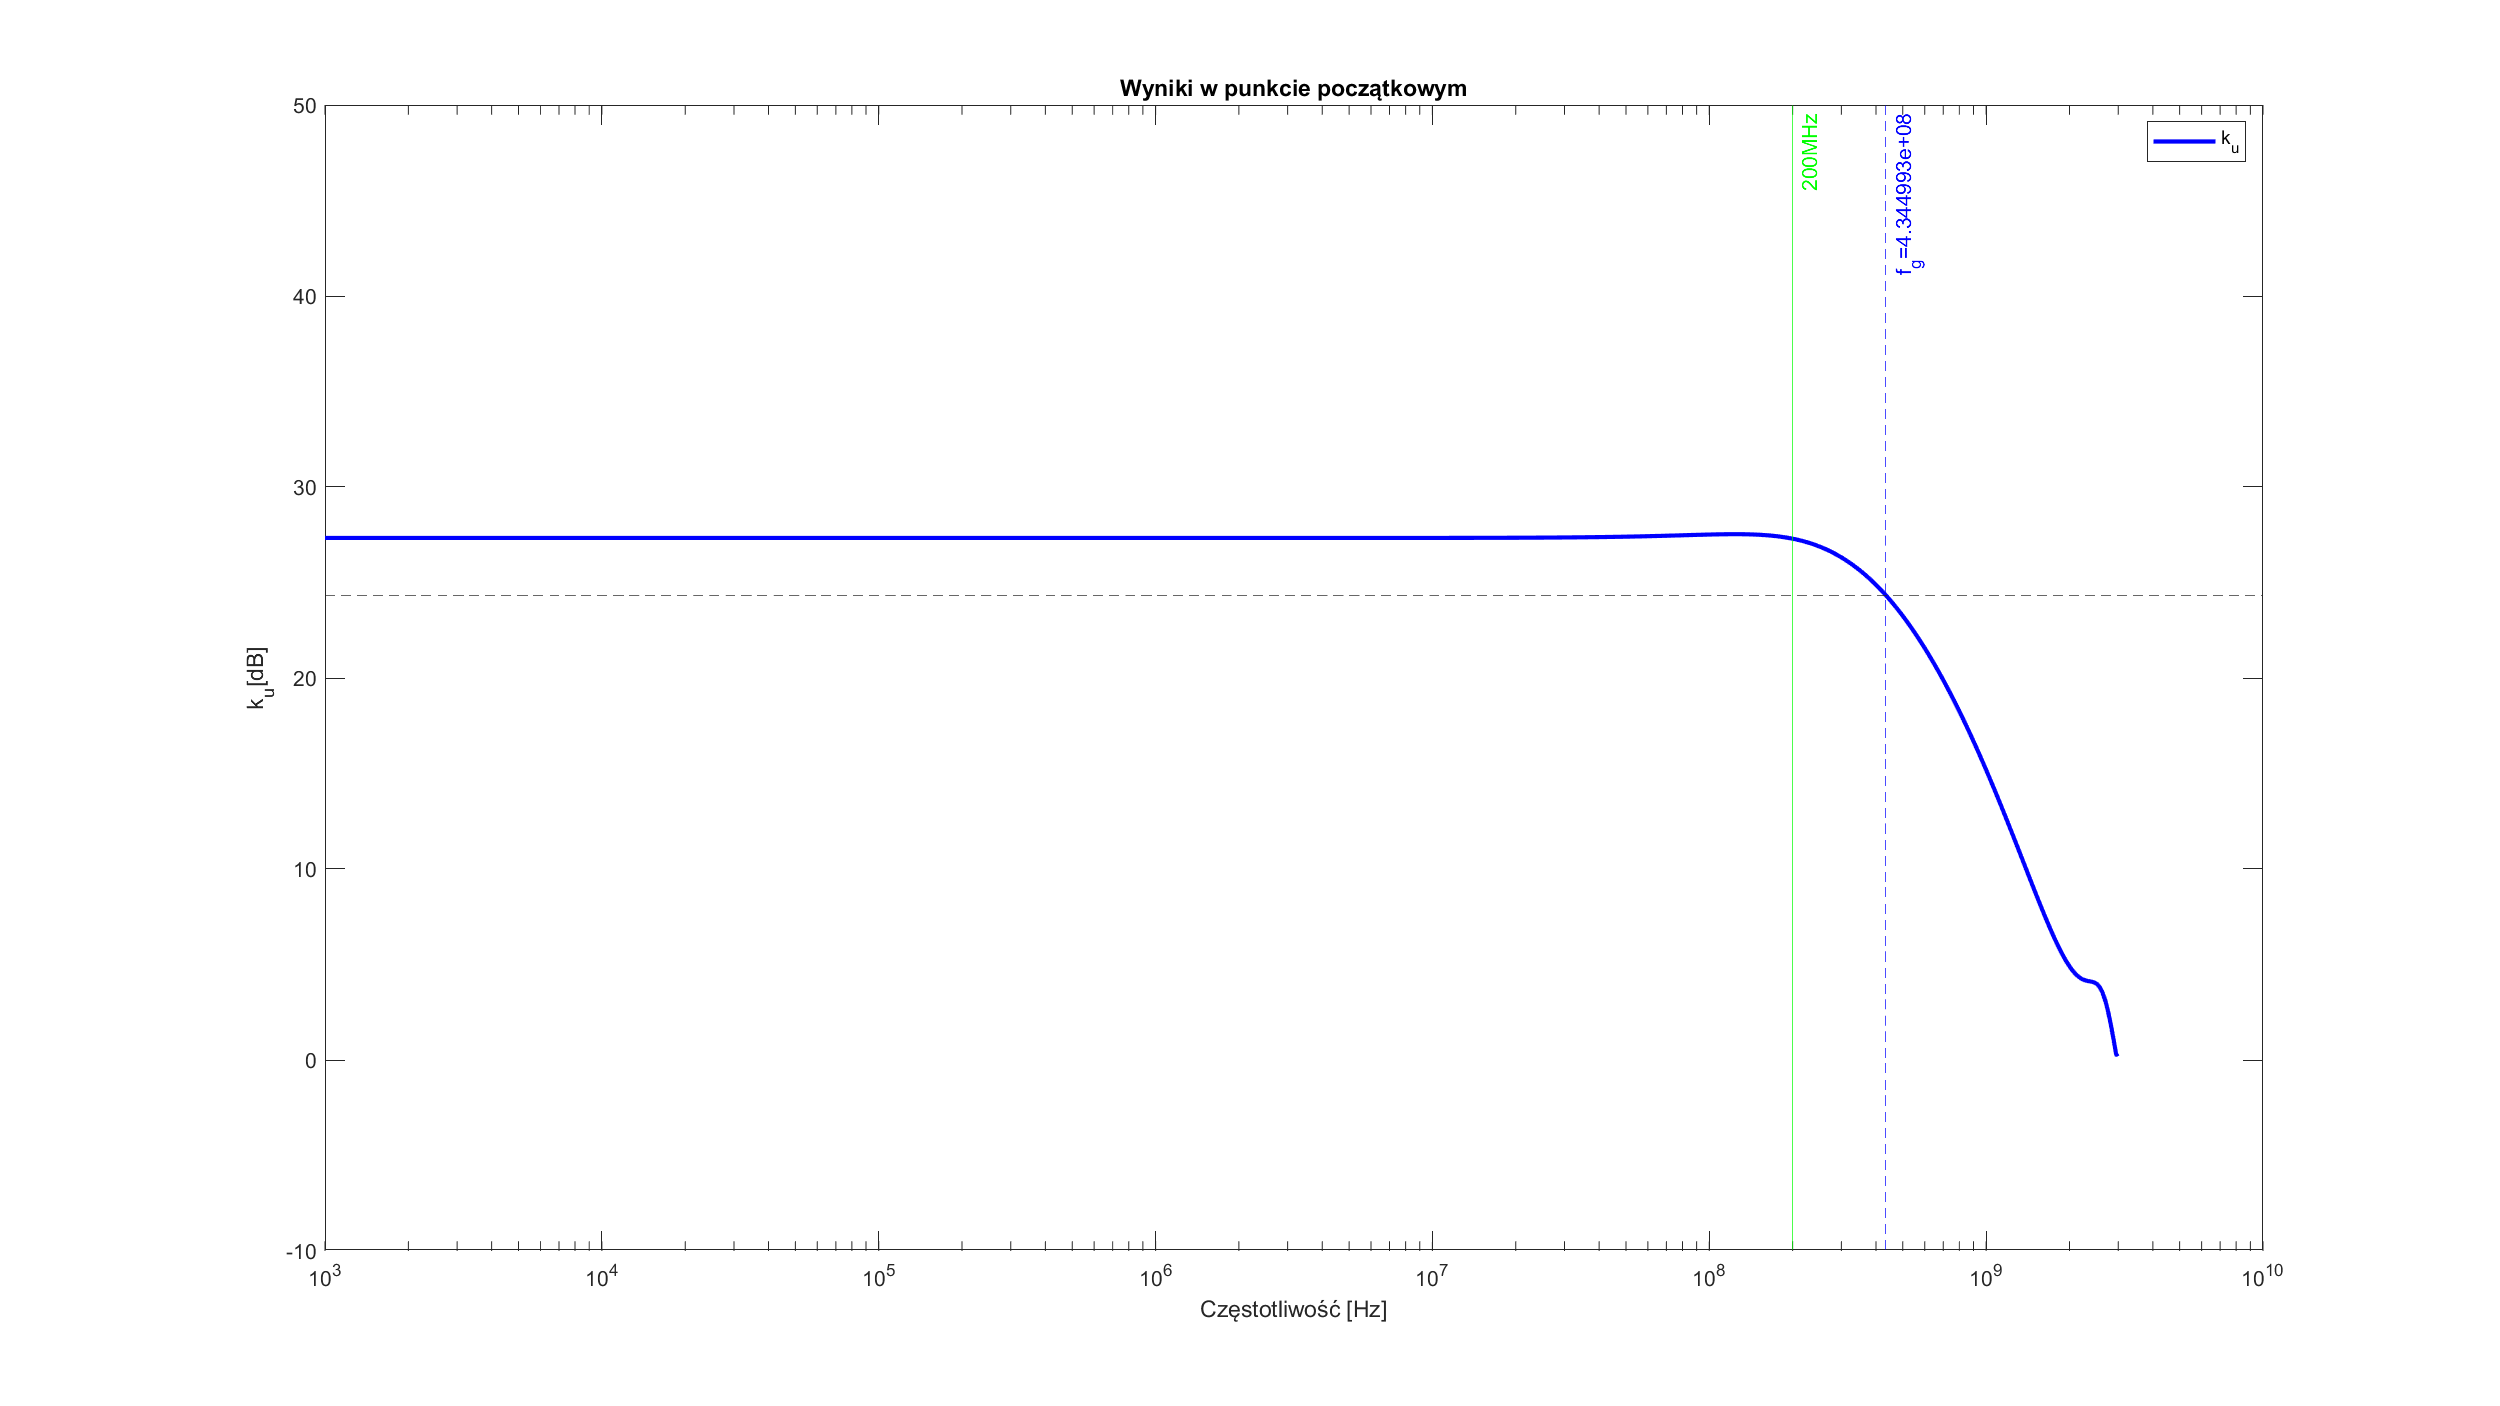
\includegraphics[width=12cm]{graphics/starting_point.png}
	\centering
	\caption{Charakterystyka układu w punkcie startowym.}
\end{figure}

Jak widać spełnione są warunki postawione w zadaniu (minimalna wartość wzmocnenia to 20 dB, przy źródle AC mającym 1V amplitudy).
\pagebreak

Aby potwierdzić, że Matlab i Spice zwracją te same wyniki przeprowadzono symulację w LTSpice:
\begin{figure}[h]
	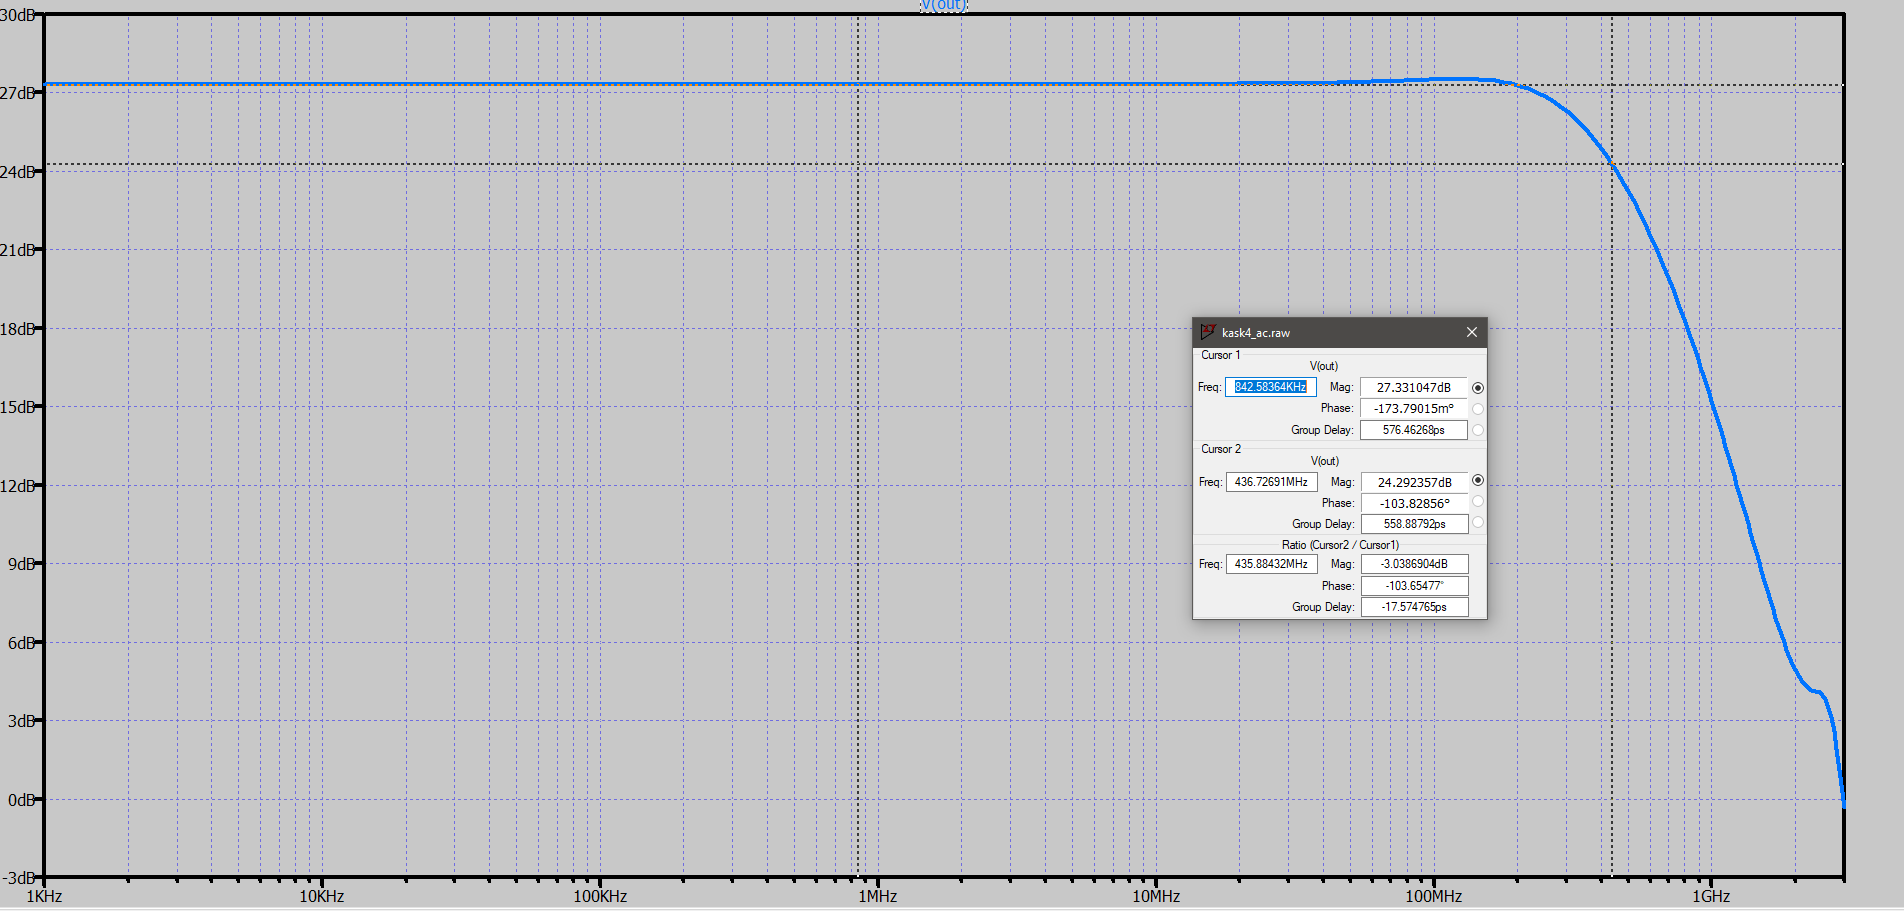
\includegraphics[width=12cm]{graphics/starting_point_spice.png}
	\centering
	\caption{Charakterystyka układu w punkcie startowym.}
\end{figure}

\subsection{Opis kodu}



\section{Metody rozwiązania numerycznego}

\pagebreak
\begin{center}
	\title{ \huge \textbf{Etap 2}}
\end{center}

\section{Funckje celu i ograniczeń, skalowanie}
\section{Wykorzystane algorytmy}
\subsection{Interior Point}
\subsubsection*{Jakość, zbieżność}
\subsection{Patternsearch}
\subsubsection*{Jakość, zbieżność}
\section{Porównanie punktu startowego, optymalnego i zbioru Pareto}
\section{Podsumowanie}
\begin{itemize}
	\item Czy zadania optymalizacji sformułwoano prawidłowo?
	      \begin{itemize}
		      \item tak
	      \end{itemize}
	\item Czy uzsykano widoczną poprawę właśności obiektu?
	      \begin{itemize}
		      \item tak
	      \end{itemize}

	\item Jaka jest złozoność obliczeniowa procesu optymalizacji?
	      \begin{itemize}
		      \item hahahah
	      \end{itemize}

\end{itemize}


\pagebreak
\begin{center}
	\title{ \huge \textbf{Wykresy w dużej rozdzielczości}}
\end{center}

\begin{landscape}
	\begin{figure}[h]
		\vspace*{-2cm}
		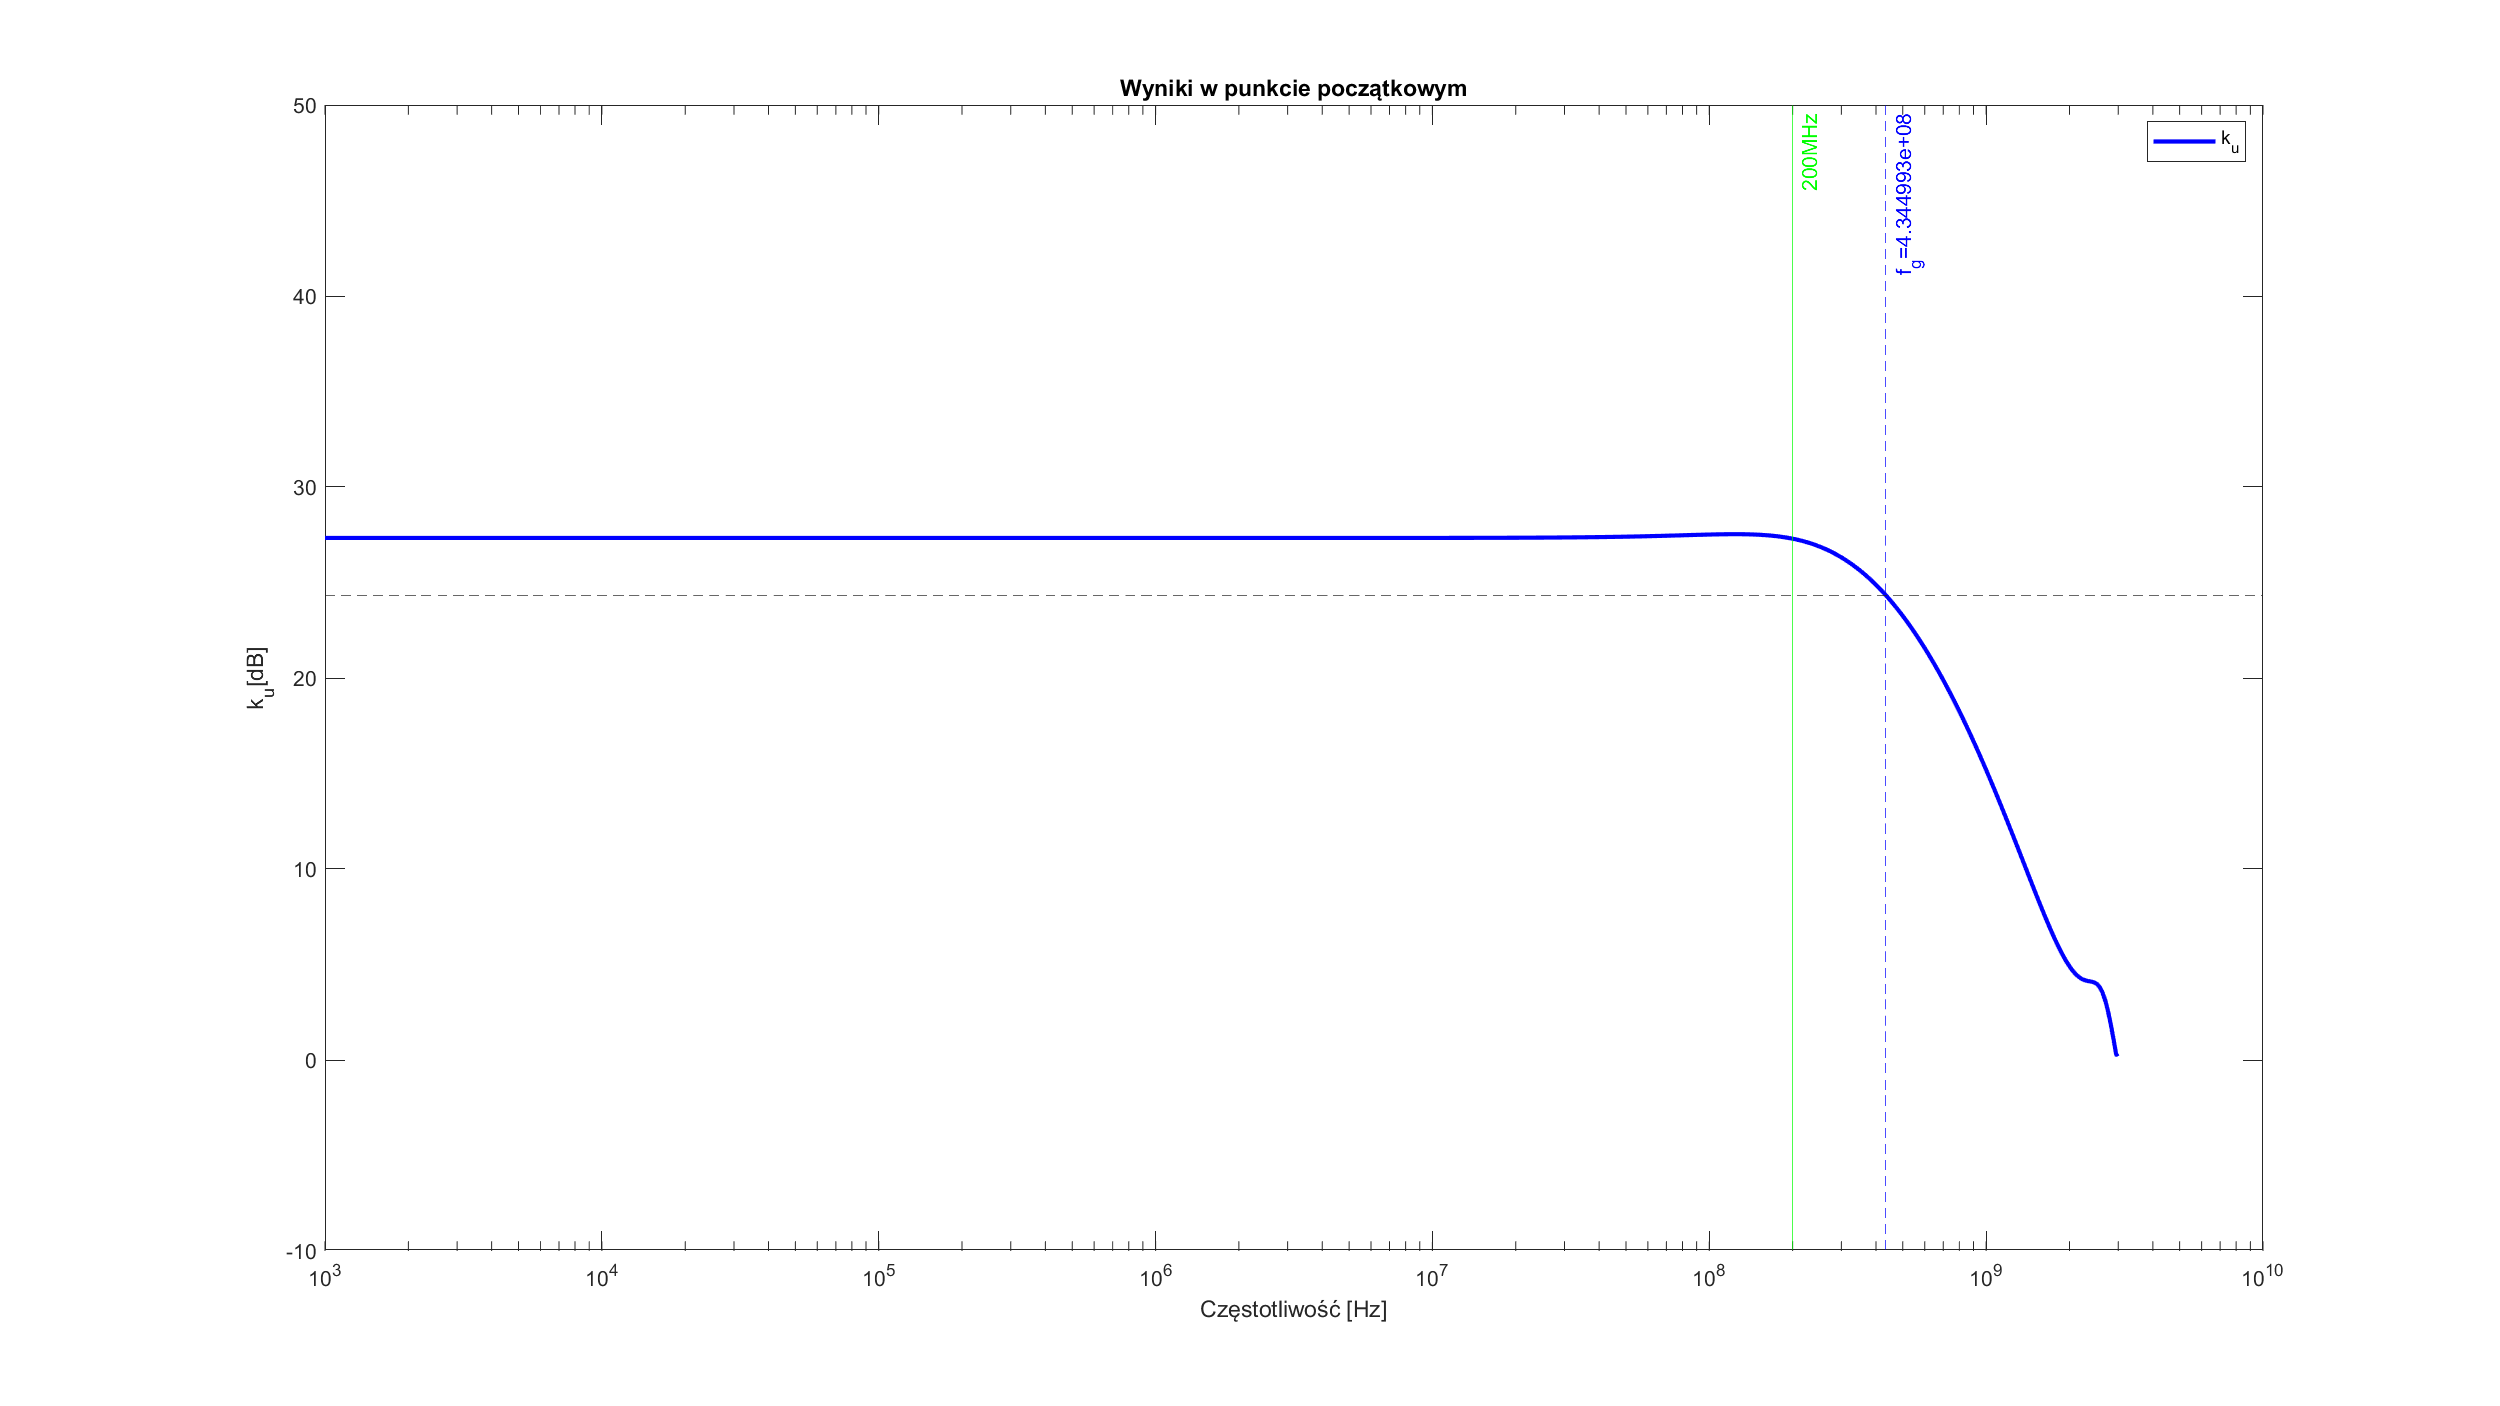
\includegraphics[width=25cm,height=15 cm]{graphics/starting_point.png}
		\centering
		\caption{Charakterystyka układu w punkcie startowym.}
	\end{figure}
\end{landscape}

\pagebreak
\begin{landscape}
	\begin{figure}[h]
		\vspace*{-2cm}
		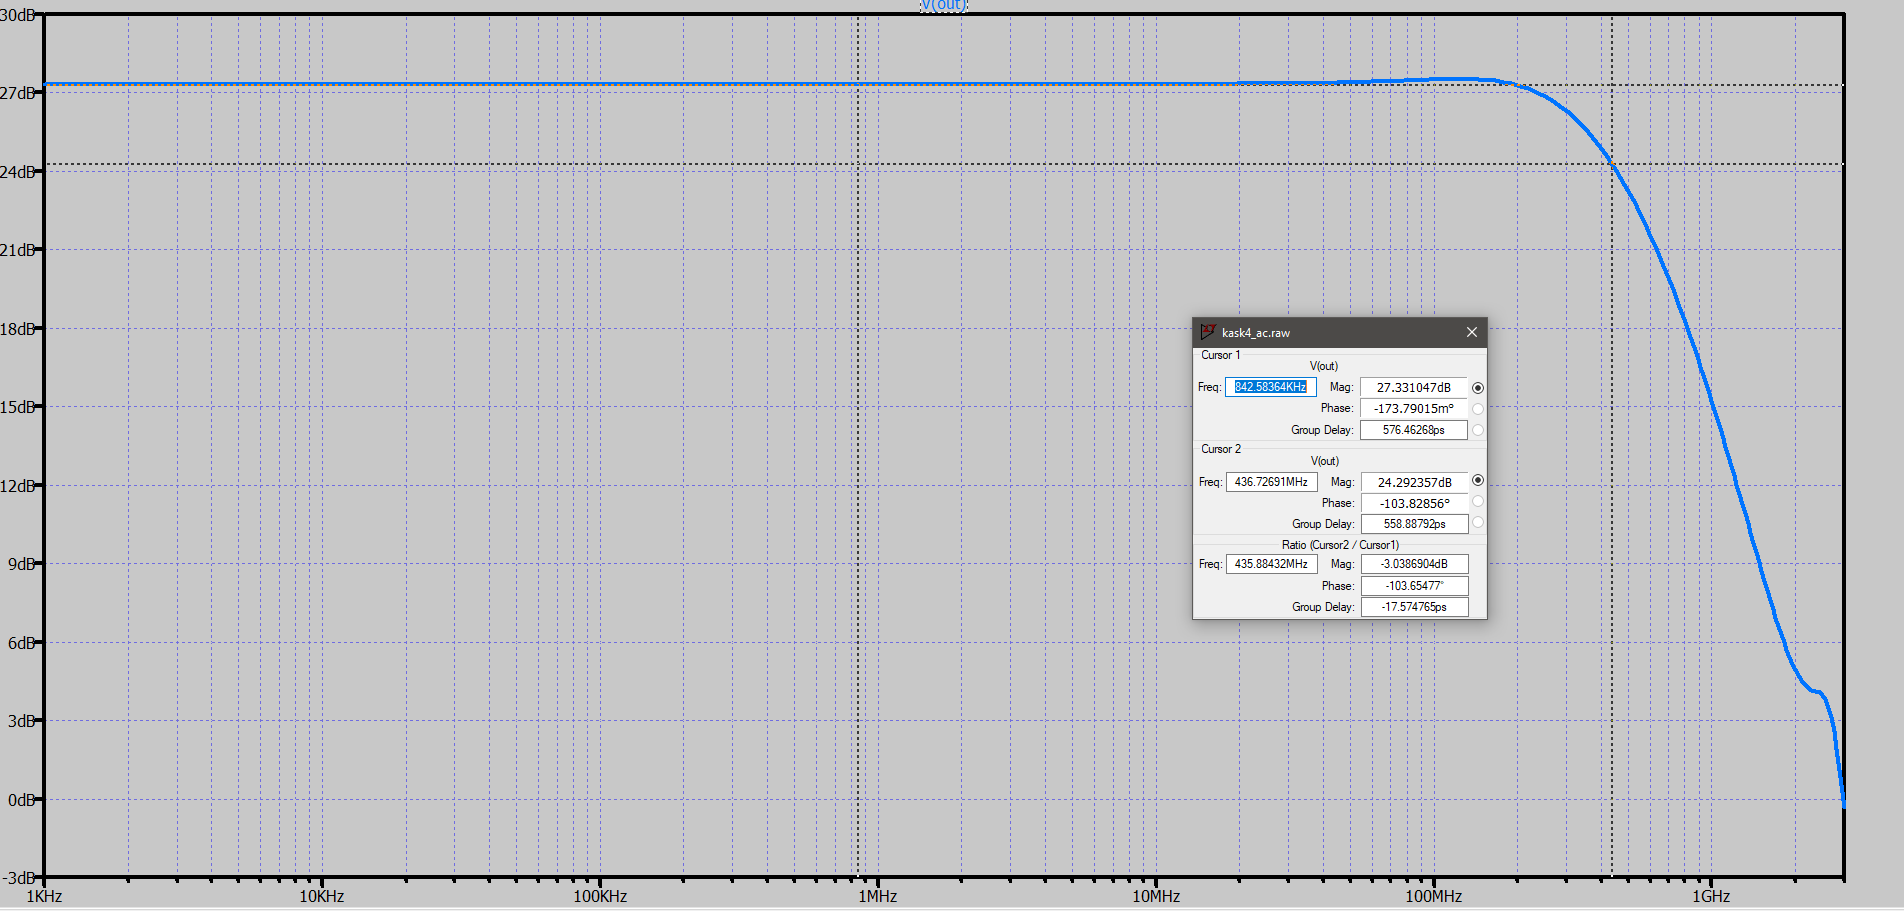
\includegraphics[width=20cm,height=10 cm]{graphics/starting_point_spice.png}
		\centering
		\caption{Charakterystyka układu w punkcie startowym (LTSpice).}
	\end{figure}
\end{landscape}

\pagebreak
\begin{landscape}
	\begin{figure}[h]
		\vspace*{-2cm}
		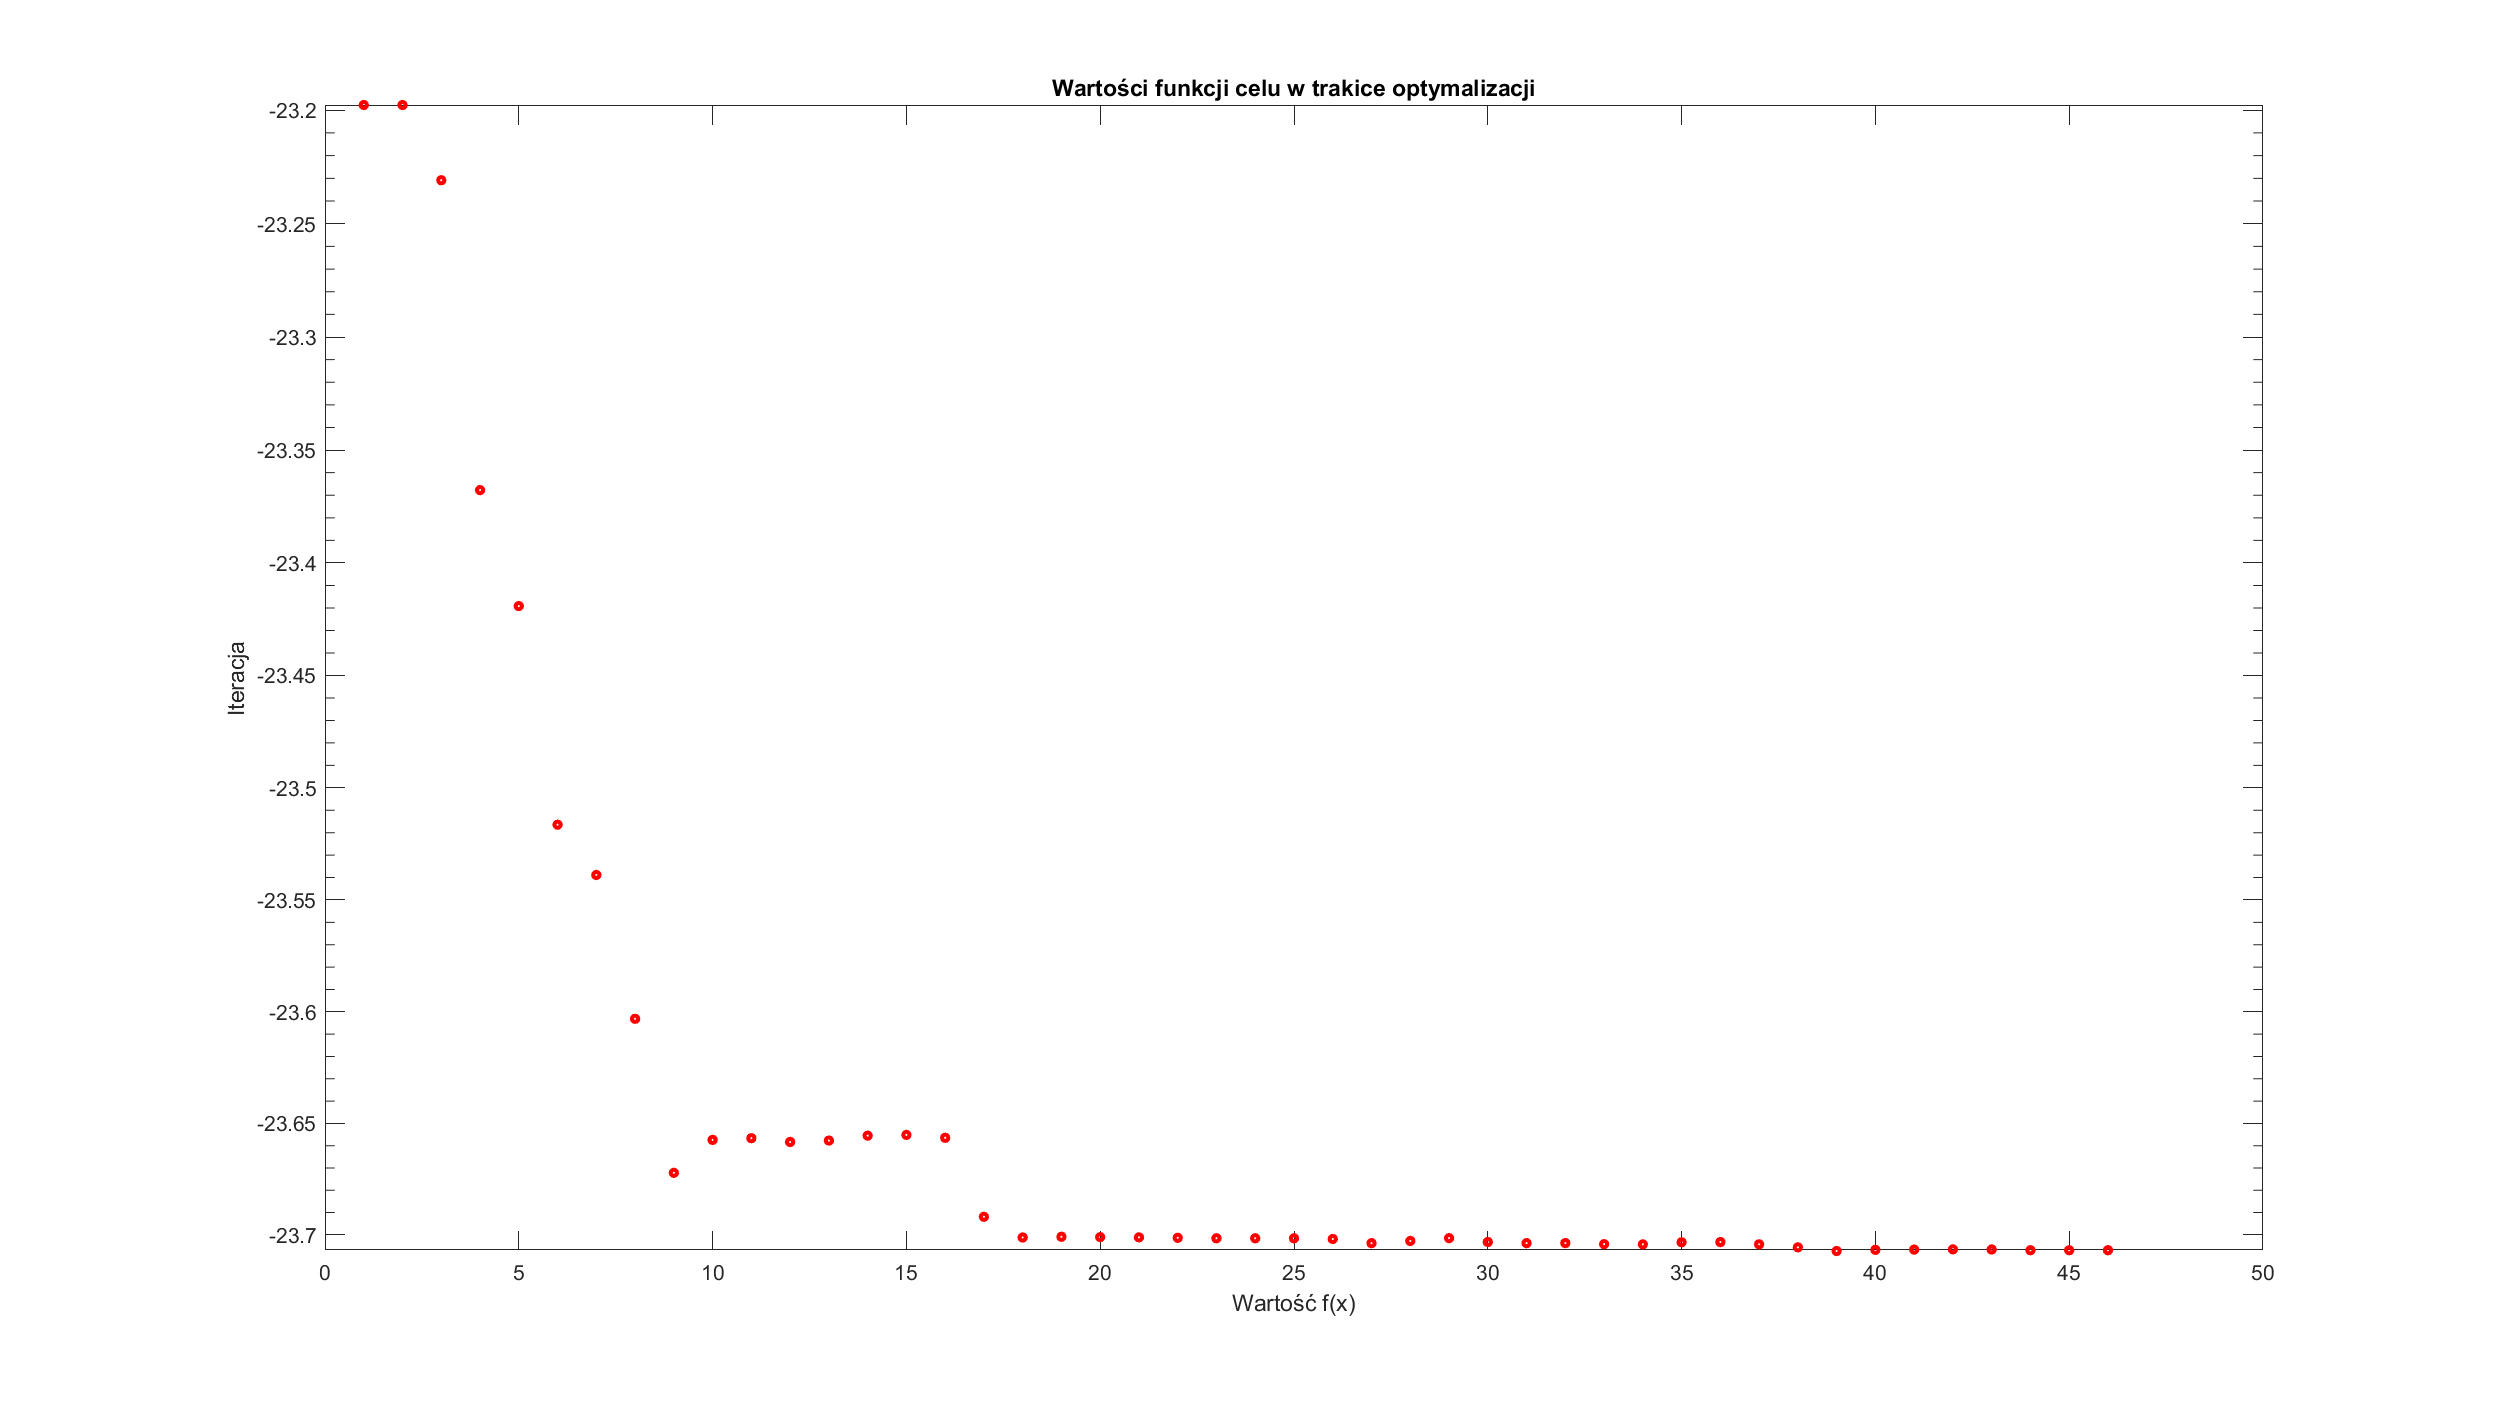
\includegraphics[width=25cm,height=15 cm]{graphics/fval.png}
		\centering
		\caption{Przebieg wartości funkcji celu.}
	\end{figure}
\end{landscape}

\pagebreak
\begin{landscape}
	\begin{figure}[h]
		\vspace*{-2cm}
		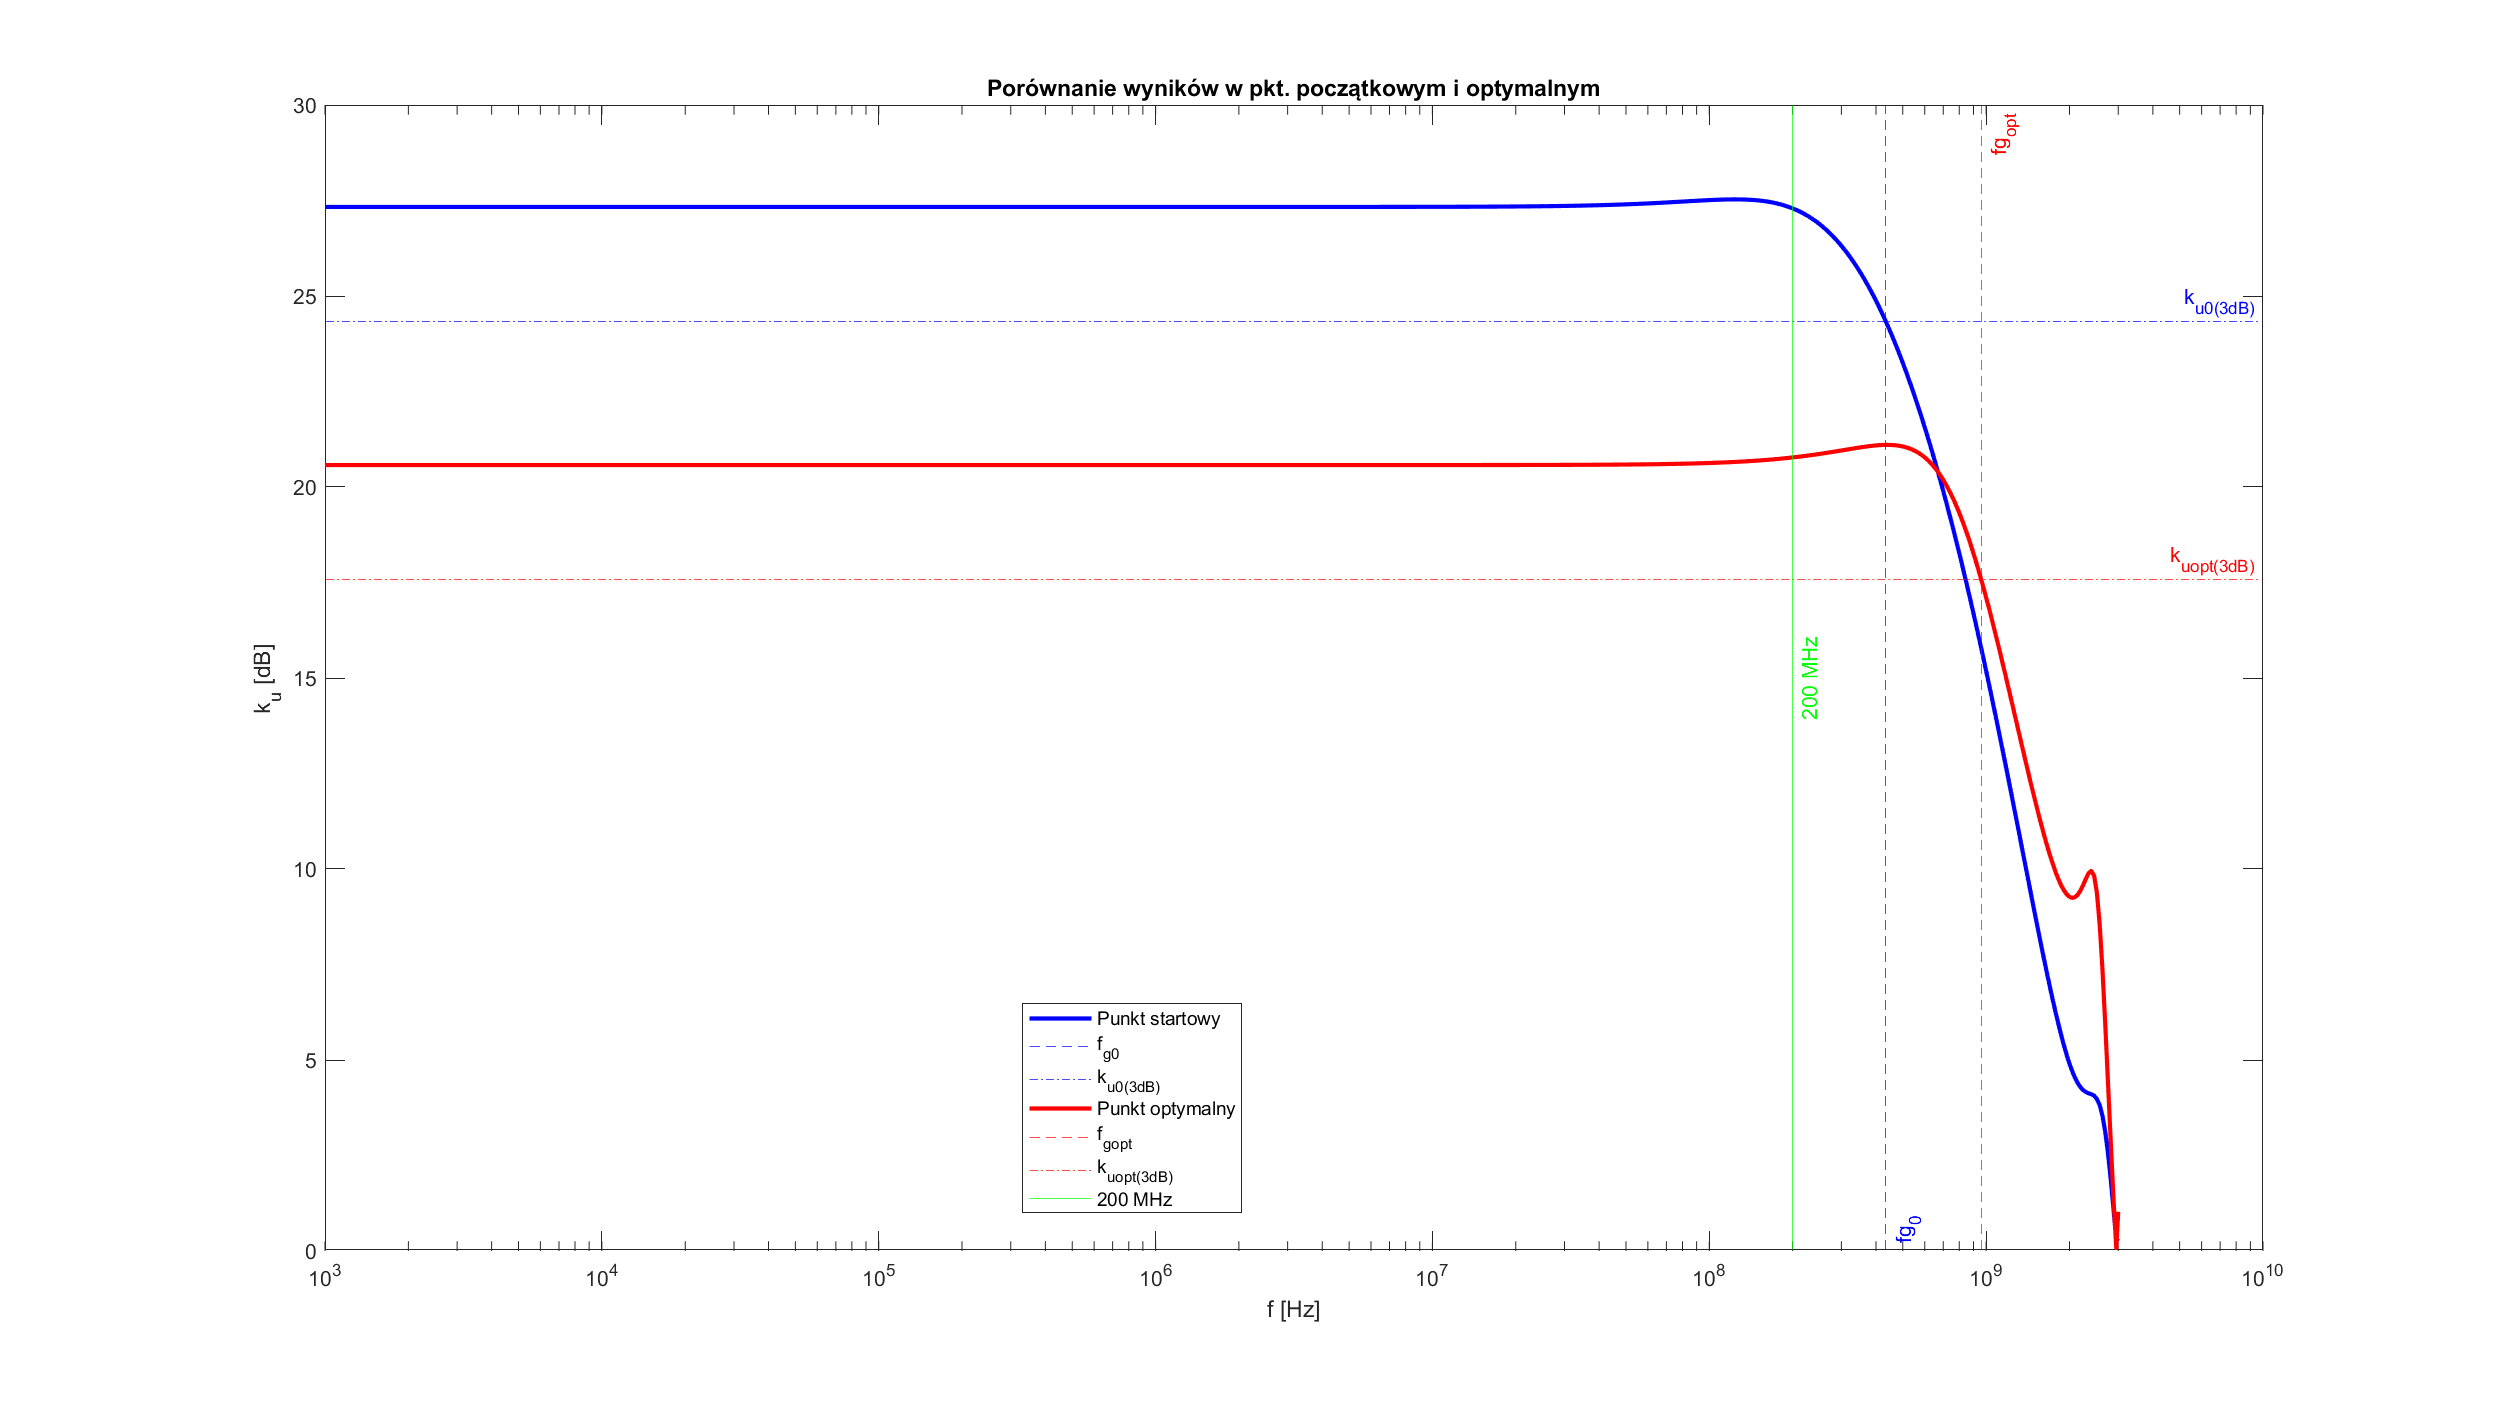
\includegraphics[width=25cm,height=15 cm]{graphics/comparison.png}
		\centering
		\caption{Porównanie wyników w punkcie optymalnym i startowym.}
	\end{figure}
\end{landscape}


\end{document}


